\documentclass[]{scrartcl}
\usepackage{graphicx}
\usepackage{geometry}
\geometry{
	a4paper,
	total={170mm,257mm},
	left=20mm,
	top=20mm,
}


%opening
\title{Software Design Description}
\author{Brandon Smith, Nieka Gutenberger, Joseph Coppin, Ryan Frazier, Trevor Jewkes}

\begin{document}

\maketitle
\pagebreak
\section{Software Design}
\subsection{Login Screen}

\centerline{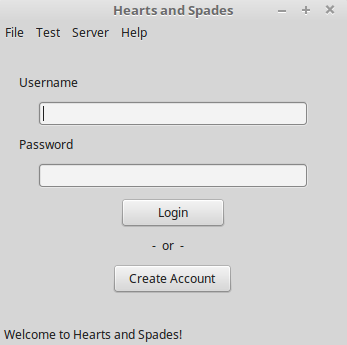
\includegraphics{LoginScreen.png}}

This screen is the first screen the user will see.  It has a text box for the user to enter a user name and password.  It also has two buttons a “login” which sends the username and password to the server, and brings up the lobby screen; and a “Create Account” button which takes the user to screen where they can create their account prior to playing games.

The account creation has text fields for all the information needed to create an account including Name, “Username”, “Password”  and “Verify Password”,  Finally the page includes a “Create Account” button which sends all information to the server so it can create the account.

\subsection{Main Menu}
\centerline{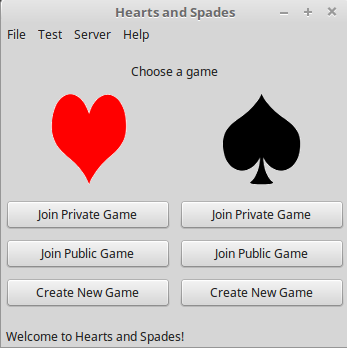
\includegraphics{SelectGame.png}}

This screen is the main menu for the Game, it is divided in half with one half related to the game of Hearts, and the other half for the game of Spades.  Each half includes three buttons, “Join Private”, “Join Public” and “Create New”.  The “Join Private” brings up a screen which allows the user enter the name of the game they want to join.  The “Join Public” will tell the server to assign the user to the first available  public game, if no game is available the server will create a new game with the user and three AI players.  Finally the “Create New” button will bring up a screen which asks for the users preferences to create a new game.

\centerline{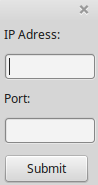
\includegraphics{ServerSelection.png}}

When connecting to the server, a menu option is available to specify the IP Address and Port number for the server.


\subsection{Game Play}
\centerline{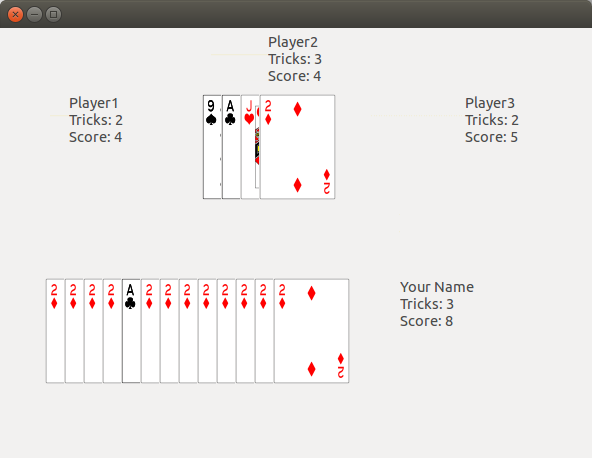
\includegraphics{game_board.png}}
This screen will be the view that will be use for play of the game. Since Spades and Hearts have the same basic set-up we can use the same view for both. It shows the players hand along with the scores of the other players. Placing bids and passing cards fit within the gameplay screen.


\subsection{End-of-Game}
\centerline{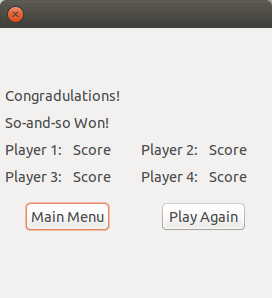
\includegraphics{end_game.png}}
This the End-of-Game screen. It will display the winner of the game along with the final scores for the game.

 There are two buttons, "Play Again" and "Main Menu". The "Play Again" button is used to play again with the same players. The "Main Menu" button will return the user to the main menu.
 


%***************************************************************************************************************//
%Hearts Section//

 \newpage
 \noindent\makebox[\textwidth{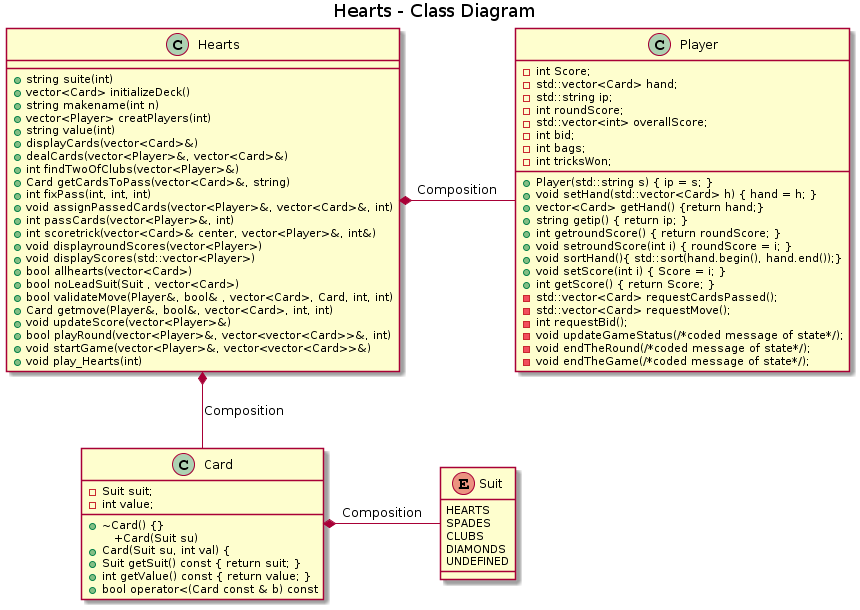
\includegraphics[width=\textwidth]{hearts.png}}]

 \section{Server Low Level Design}

\subsection{Hearts Class}
 \begin{itemize}
 	\item string suite(int i)
 		\begin{itemize}
 			\item Converts enum of ints to string of card suit.
 		\end{itemize}
 	\item vector $\langle$Card$\rangle$ initializeDeck()
 		\begin{itemize}
 			\item Creates deck of cards taken from card class.
 		\end{itemize}
 	\item string makename(int n)
 		\begin{itemize}
 			\item 	Creates a player name.
 		\end{itemize}
 	\item vector$\langle$Player$\rangle$  creatPlayers(int p)
 		\begin{itemize}
 			\item Creates a vector of Players to play the game.
 		\end{itemize}
 	\item void displayCards(vector$\langle$Card$\rangle$ \& hand)
 		\begin{itemize}
 			\item Displays the deck for screen purposes.
 		\end{itemize}
 	\item void dealCards(vector$\langle$Player$\rangle$ \& players, vector$\langle$Card$\rangle$ \& Deck)
 		\begin{itemize}
 			\item Deals cards to players.
 		\end{itemize}
 	\item int findTwoOfClubs(vector$\langle$Player$\rangle$ \& p)
 		\begin{itemize}
 			\item Looks through each hand to find the 2 of clubs to find starting player and hand.
 		\end{itemize}
 	\item Card getCardsToPass(vector$\langle$Card$\rangle$ \& h, string p)
 		\begin{itemize}
 			\item Gets and stores cards for passing at the beginning of each round.
 		\end{itemize}
 	\item int fixPass(int r, int p, int c)
 		\begin{itemize}
 			\item Ensures that cards are passed to the right players depending on the round.
 		\end{itemize}
 	\item void assignPassedCards(vector$\langle$Player$\rangle$ \& p, vector$\langle$Card$\rangle$ \& h, int r)
 		\begin{itemize}
 			\item Takes the passed cards and redistributes based on round.
 		\end{itemize}
 	\item int passCards(vector$\langle$Player$\rangle$ \& p, int round)
 		\begin{itemize}
 			\item Function for passing cards at beginging of round.
 		\end{itemize}
 	\item int scoretrick(vector$\langle$Card$\rangle$ \& center, vector$\langle$Player$\rangle$ \& players, int\& turn)
 		\begin{itemize}
 			\item 	Holds the score for the current trick.
 		\end{itemize}
 	\item void displayroundScores(vector$\langle$Player$\rangle$ p)
 		\begin{itemize}
 			\item Displays scores for the round.
 		\end{itemize}
 	\item void displayScores(vector$\langle$Player$\rangle$  p)
 		\begin{itemize}
 			\item Display scores each turn.
 		\end{itemize}
 	\item bool allhearts(vector$\langle$Card$\rangle$ h)
 		\begin{itemize}
 			\item Checks to see if a players hand is all hearts.
 		\end{itemize}
 	\item string value(int i)
 	\item bool noLeadSuit(Suit s, vector$\langle$Card$\rangle$ h)
 		\begin{itemize}
 			\item Compares hand against the lead suit
 		\end{itemize}
 	\item bool validateMove(Player\& p, bool\& broken, vector$\langle$Card$\rangle$  Center, Card move, int t, int i)
 	\item Card getmove(Player\& p, bool\& b, vector$\langle$Card$\rangle$  c, int t, int i)
 	\item void updateScore(vector$\langle$Player$\rangle$ \& p)
 		\begin{itemize}
 			\item Adds round score to Score.
 		\end{itemize}
 	\item bool playRound(vector$\langle$Player$\rangle$ \& players, vector$\langle$vector$\langle$Card$\rangle$ $\rangle$\& history, int round)
 	\item void startGame(vector$\langle$Player$\rangle$ \& players, vector$\langle$vector$\langle$Card$\rangle$ $\rangle$\& history)
 		\begin{itemize}
 			\item  Uses players and calls round until game is over
 		\end{itemize}
 	\item void play\_Hearts(int num)

 \end{itemize}

 %***************************************************************************************************************//
 %Client Section//
\newpage

 \centerline{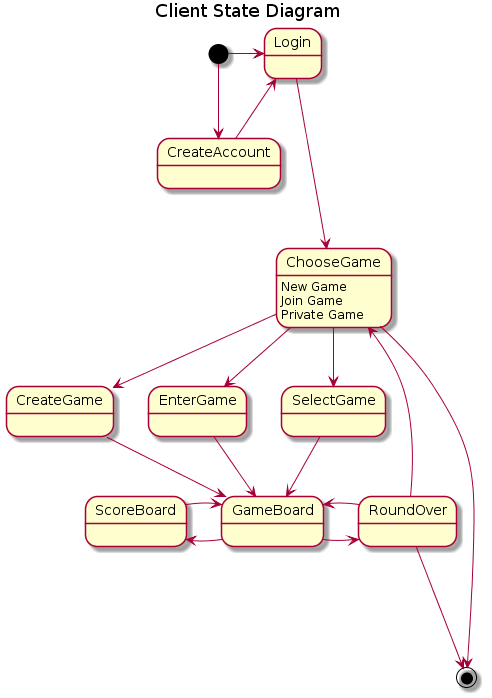
\includegraphics{Client State Diagram.png}}
 \noindent\makebox[\textwidth{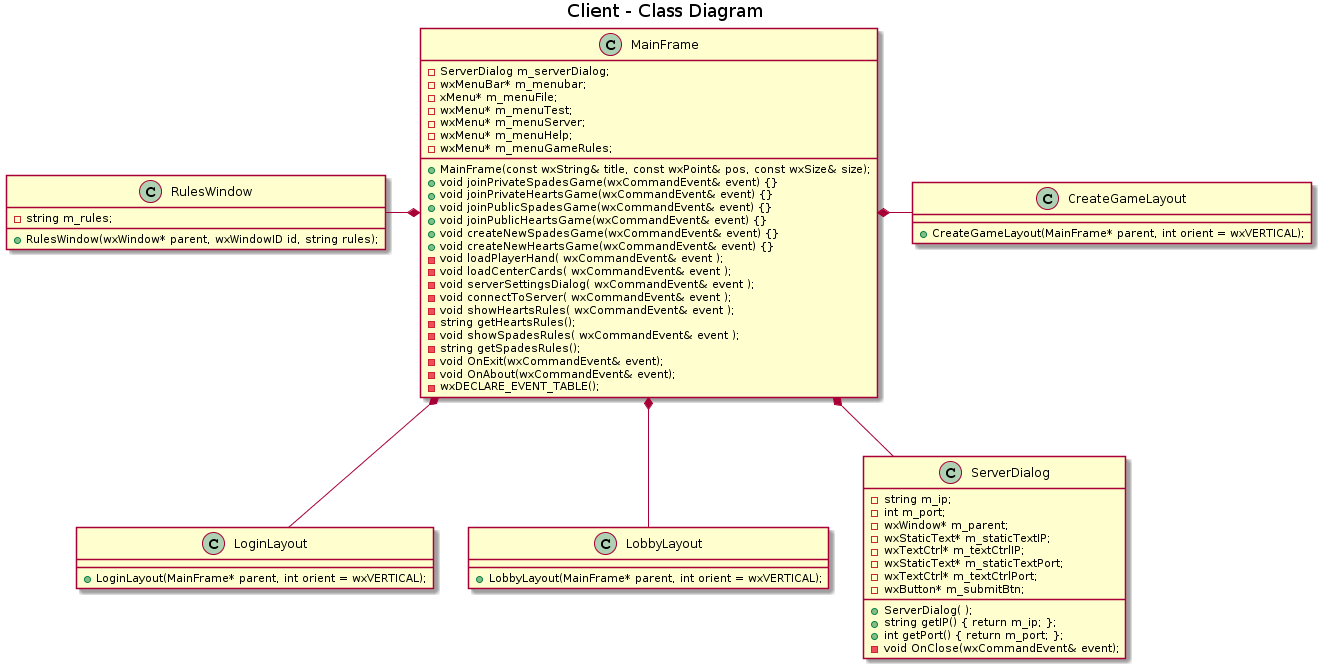
\includegraphics[width=\textwidth]{clientClassDiagram.png}}]

 \section{Client Low-Level Design }
 
 \subsection{MainFrame}
 	This class is inherited publically from wxFrame.

 	\begin{itemize}
 		\item public:

 		\begin{itemize}
 			\item MainFrame(const wxString\& title, const wxPoint\& pos, const wxSize\& size);
 				\\ In the main frame, the main components of the software are held. Following are the functions included:

 			\item void joinPrivateSpadesGame(wxCommandEvent\& event) {}
 				\\This function allows a user to join a spades game that is closed to public use.

 			\item void joinPrivateHeartsGame(wxCommandEvent\& event) {}
 				\\ This function allows a user to join a hearts game that is closed to public view.

 			\item void joinPublicSpadesGame(wxCommandEvent\& event) {}
 				\\ This function will allow user to connect to first available spades game.

 			\item void joinPublicHeartsGame(wxCommandEvent\& event) {}
 				\\ This function will allow user to connect to first available hearts game.

 			\item void createNewSpadesGame(wxCommandEvent\& event) {}
 				\\	This function will create a new Spades Game.

 			\item void createNewHeartsGame(wxCommandEvent\& event) {}
 				\\ This function will create a new Hearts Game.

 		\end{itemize}

 		\item 	private:

 		\begin{itemize}
 			\item ServerDialog m\_serverDialog;
 			\item wxMenuBar* m\_menubar;
 			\item xMenu* m\_menuFile;
 			\item wxMenu* m\_menuServer;
 			\item wxMenu* m\_menuHelp;
 			\item wxMenu* m\_menuGameRules;
 			\item void loadPlayerHand( wxCommandEvent\& event );
 				\\Allows for players hand to be loaded on screen from server.
 			\item void loadCenterCards( wxCommandEvent\& event );
 				\\Allows for cards to be placed in middle of screen after play.
 			\item void serverSettingsDialog( wxCommandEvent\& event );
 			\item void connectToServer( wxCommandEvent\& event );
 				\\Allows player to connect to server to play game of choice.
 			\item void showHeartsRules( wxCommandEvent\& event );
 				\\Allows user to get Hearts Rules.
 			\item std::string getHeartsRules();
 			\item void showSpadesRules( wxCommandEvent\& event );
 				\\Allows user to get Spades Rules.
 			\item std::string getSpadesRules();
 			\item void OnExit(wxCommandEvent\& event);
 				\\Allows user to exit program.
 			\item void OnAbout(wxCommandEvent\& event);
 				\\Allows user to see details of program.
 			\item wxDECLARE\_EVENT\_TABLE();
 		\end{itemize}
 	\end{itemize}


 \subsection{ServerDialog }
 	This class is inherited publically from wxDialog.
 	\begin{itemize}
 	\item public:

 	\begin{itemize}
 		\item ServerDialog( wxWindow* parent, wxWindowID id = wxID\_ANY, const wxString\& title = wxEmptyString, const wxPoint\& pos = wxDefaultPosition, const wxSize\& size = wxDefaultSize, long style = wxDEFAULT\_DIALOG\_STYLE );

 		\item std::string getIP() { return m\_ip; };

 		\item int getPort() { return m\_port; };
 	\end{itemize}

 	\item private:
 	\item protected:
 		\begin{itemize}
 			\item std::string m\_ip;
 			\item	int m\_port;
 			\item	wxWindow* m\_parent;
 			\item	wxStaticText* m\_staticTextIP;
 			\item	wxTextCtrl* m\_textCtrlIP;
 			\item	wxStaticText* m\_staticTextPort;
 			\item	wxTextCtrl* m\_textCtrlPort;
 			\item	wxButton* m\_submitBtn;
 			\item	void OnClose(wxCommandEvent\& event);
 		\end{itemize}
 	\end{itemize}

 \subsection{RulesWindow }
 	This class is inherited  publically from wxScrolledWindow

 	\begin{itemize}
 		\item 	public:
 		\begin{itemize}
 			\item RulesWindow(wxWindow* parent, wxWindowID id, std::string rules);
 				\\This allows user to read and learn rules for either Hearts or Spades.
 		\end{itemize}
 	\end{itemize}

 	\begin{itemize}
 		\item 	private:
 		\begin{itemize}
 			\item std::string m\_rules;
 		\end{itemize}
 	\end{itemize}


 \subsection{LoginLayout }
 	This class is inherited  publically from wxBoxSizer
 	\begin{itemize}
 		\item public:
 		\begin{itemize}
 			\item	LoginLayout(MainFrame* parent, int orient = wxVERTICAL);
 				\\This function will bring up a screen where user may login to play game.
 		\end{itemize}
 	\end{itemize}



 \subsection{LobbyLayout}
 	This class is inherited  publically from wxBoxSizer
 		\begin{itemize}
 			\item public:
 			\begin{itemize}
 				\item	LobbyLayout(MainFrame* parent, int orient = wxVERTICAL);
 					\\This function allows the user to access the game lobby.
 			\end{itemize}
 		\end{itemize}

 \subsection{CreateGameLayout}
 	This class is inherited  publically from wxBoxSizer

 		\begin{itemize}
 			\item public:
 			\begin{itemize}
 				\item	CreateGameLayout(MainFrame* parent, int orient = wxVERTICAL);
 					\\When called, this function sets up a game layout for game play.
 			\end{itemize}
 		\end{itemize}

\end{document}
